\section{Performance and Experimental Challenges}
\label{sec:performance_and_challenges}

\subsection{Performance of the spherical harmonics analysis on 0{\nbb} decay and $^{8}$B events.}

Comparison of $S_0$ and $S_1$ distributions between 0{\nbb} decay and
$^{8}$B events is shown in Fig.~\ref{fig:S_vs_energy}. There is a
noticeable separation between the signal and background. We also note
that in the energy range of interest $S_l$'s do not have strong
dependence on the energy deposited in the detector, which makes them
reliable discriminators at the end point of the 0{\nbb} decay energy
spectrum. The information about the event topology is complimentary to
the energy measurements.

\begin{figure*}[h]
\centering
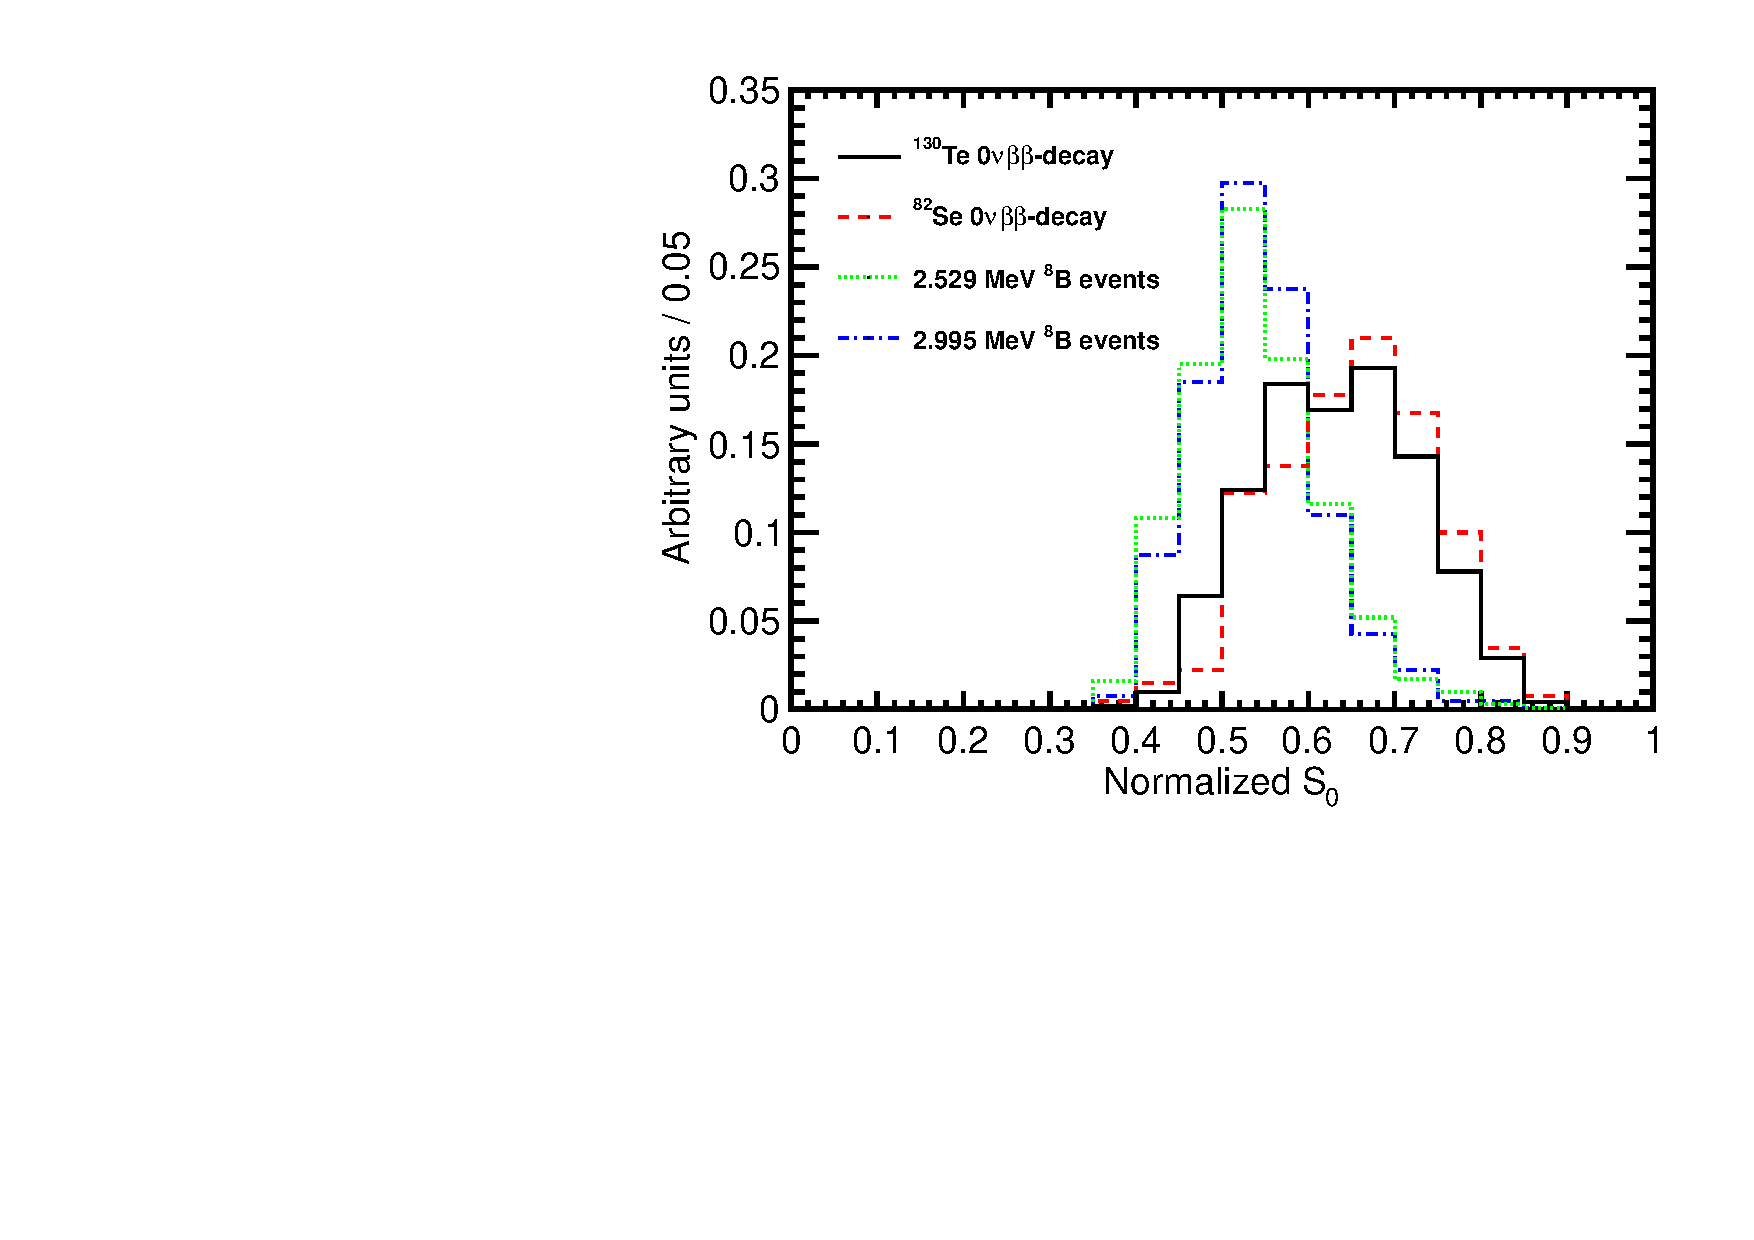
\includegraphics[width=0.49\textwidth]{hS0.pdf}
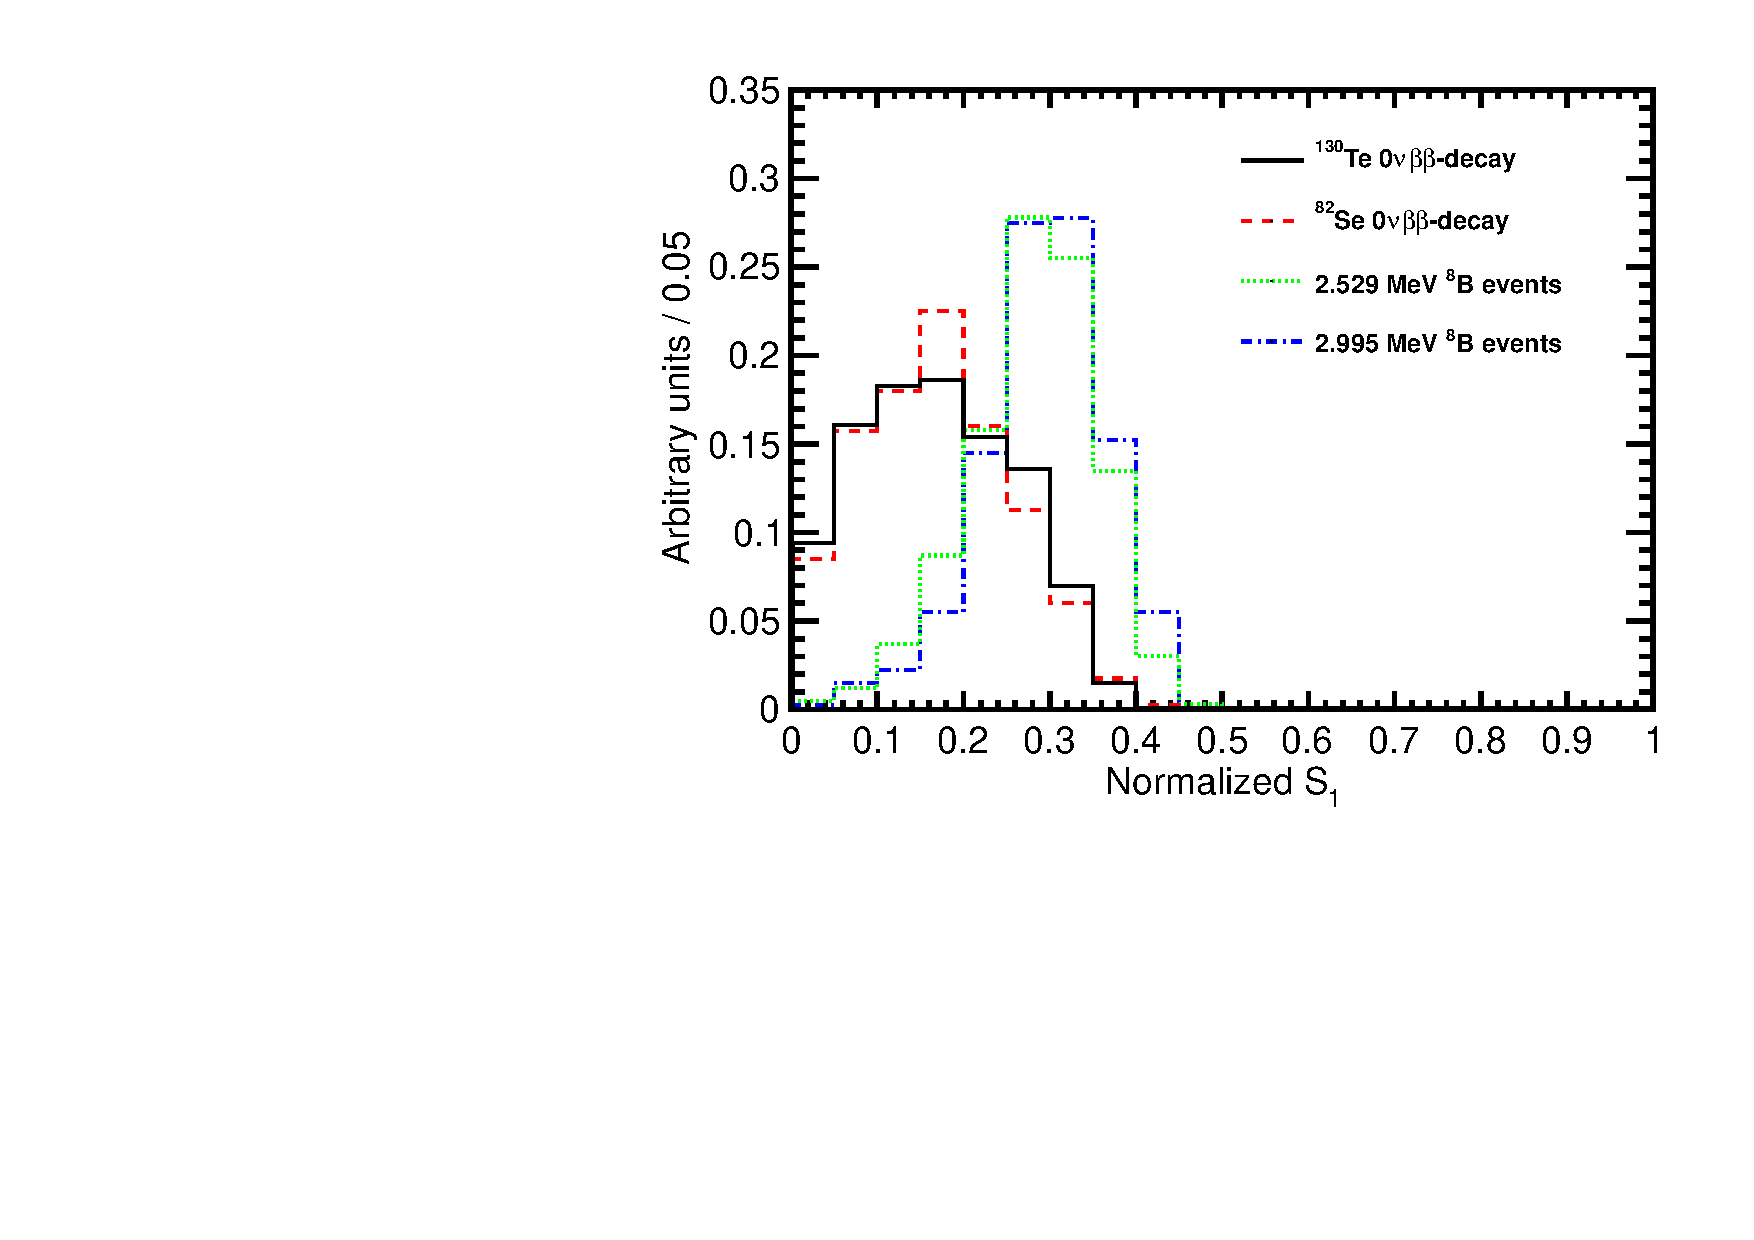
\includegraphics[width=0.49\textwidth]{hS1.pdf}
\caption{$S_0$ (\emph{left}) and $S_1$ (\emph{right}) distributions
  for events with two different event topologies and total kinetic
  energy. $^{130}$Te, $^{82}$Se 0{\nbb} decay, 2.529 MeV and 2.995 MeV
  events are compared. The simulation is done for events with the
  vertex in the center of the detector. $^{8}$B events are implemented
  as 2.529~MeV or 2.995~MeV electrons with initial direction along
  $x$-axis. Perfect vertex reconstruction - true vertex position is
  used. Time cut of 33.5~ns on the photon arrival time is applied.}
\label{fig:S_vs_energy}
\end{figure*}

Figure~\ref{fig:SL_Te_33p5ns_center} shows separation between
$^{130}$Te signal and $^{8}$B background events simulated at the
center of the detector. True values of vertex position and time is
used. Time cut of 33.5~ns on the photon arrival time is applied to
separate Cherenkov and scintillation light. Most of the discrimination
between signal and background comes from $S_0$ and $S_1$. In the
following $S_2$ and $S_3$ are not used to separate $^{130}$Te and
$^{8}$B events\footnote{$S_2$ and $S_3$ are helpful for separation of
  $^{130}$Te signal from $^{10}$C background. See Appendix.}. The
scatter plot of $S_2$ vs $S_3$ is shown here for completeness.

In order to optimize separation between $^{130}$Te signal and $^{8}$B
background a linear combination of $S_0$ and $S_1$, $S_{01}$, is
used. A linear fit, $S_0$ = $A \times S_1 + B$, of 2-dimensional $S_0$
vs $S_1$ scatter plot is performed as shown in
Fig.~\ref{fig:SL_Te_33p5ns_center}. Then this 2-dimensional
distribution is projected onto the fitted line. {\bf A little bit of
  math here to quantitatively describe $S_{01}$ via $S_0$ and $S_1$:}
A new coordinate frame is obtained by rotation of the original
$S_0$-$S_1$ frame at angle $\theta$ obtained from the fit:
$tan(\theta)$=$A$. A transformation, $S_{01} = S_1 \cdot cos(\theta) +
S_0 \cdot sin(\theta)$, defines the $S_{01}$ variable.

Bottom plot in Fig.~\ref{fig:SL_Te_33p5ns_center} shows performance of
the $S_{01}$ variable to separate $^{130}$Te signal and $^{8}$B
background. A fit to this distribution can be done to optimize the
discrimination power in a particular experimental settings. Here we
refrain from quantitative estimates on the improvements in sensitivity
to 0{\nbb} decay search using this method of spherical harmonics as a
reliable estimate would require a dedicated analysis taking into
account all the details of a particular experiment.

\begin{figure*}[h]
  \centering
  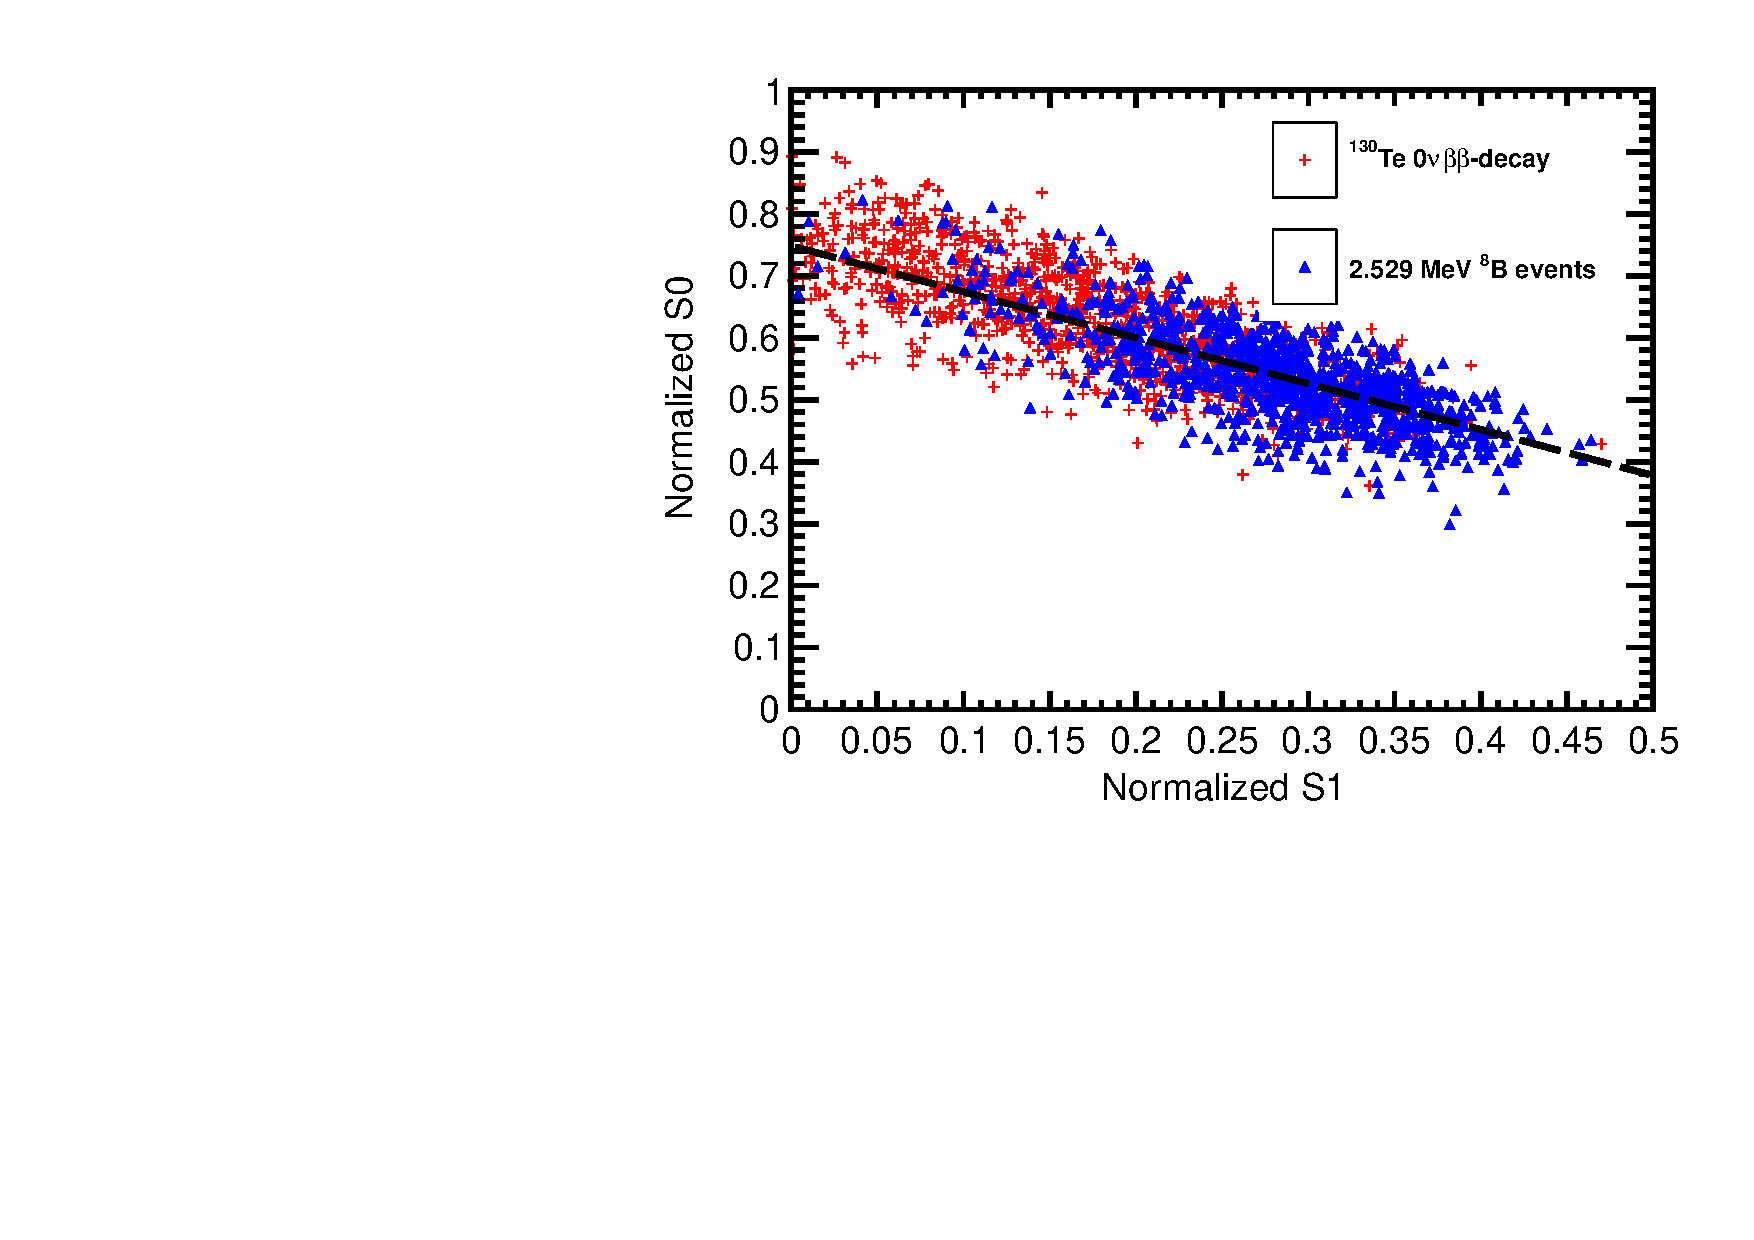
\includegraphics[width=0.49\textwidth]{hS0vsS1_Te130_1el_allLight_VtxSmear0cm_VtxShiftX0cm_33p5ns_center.pdf}
  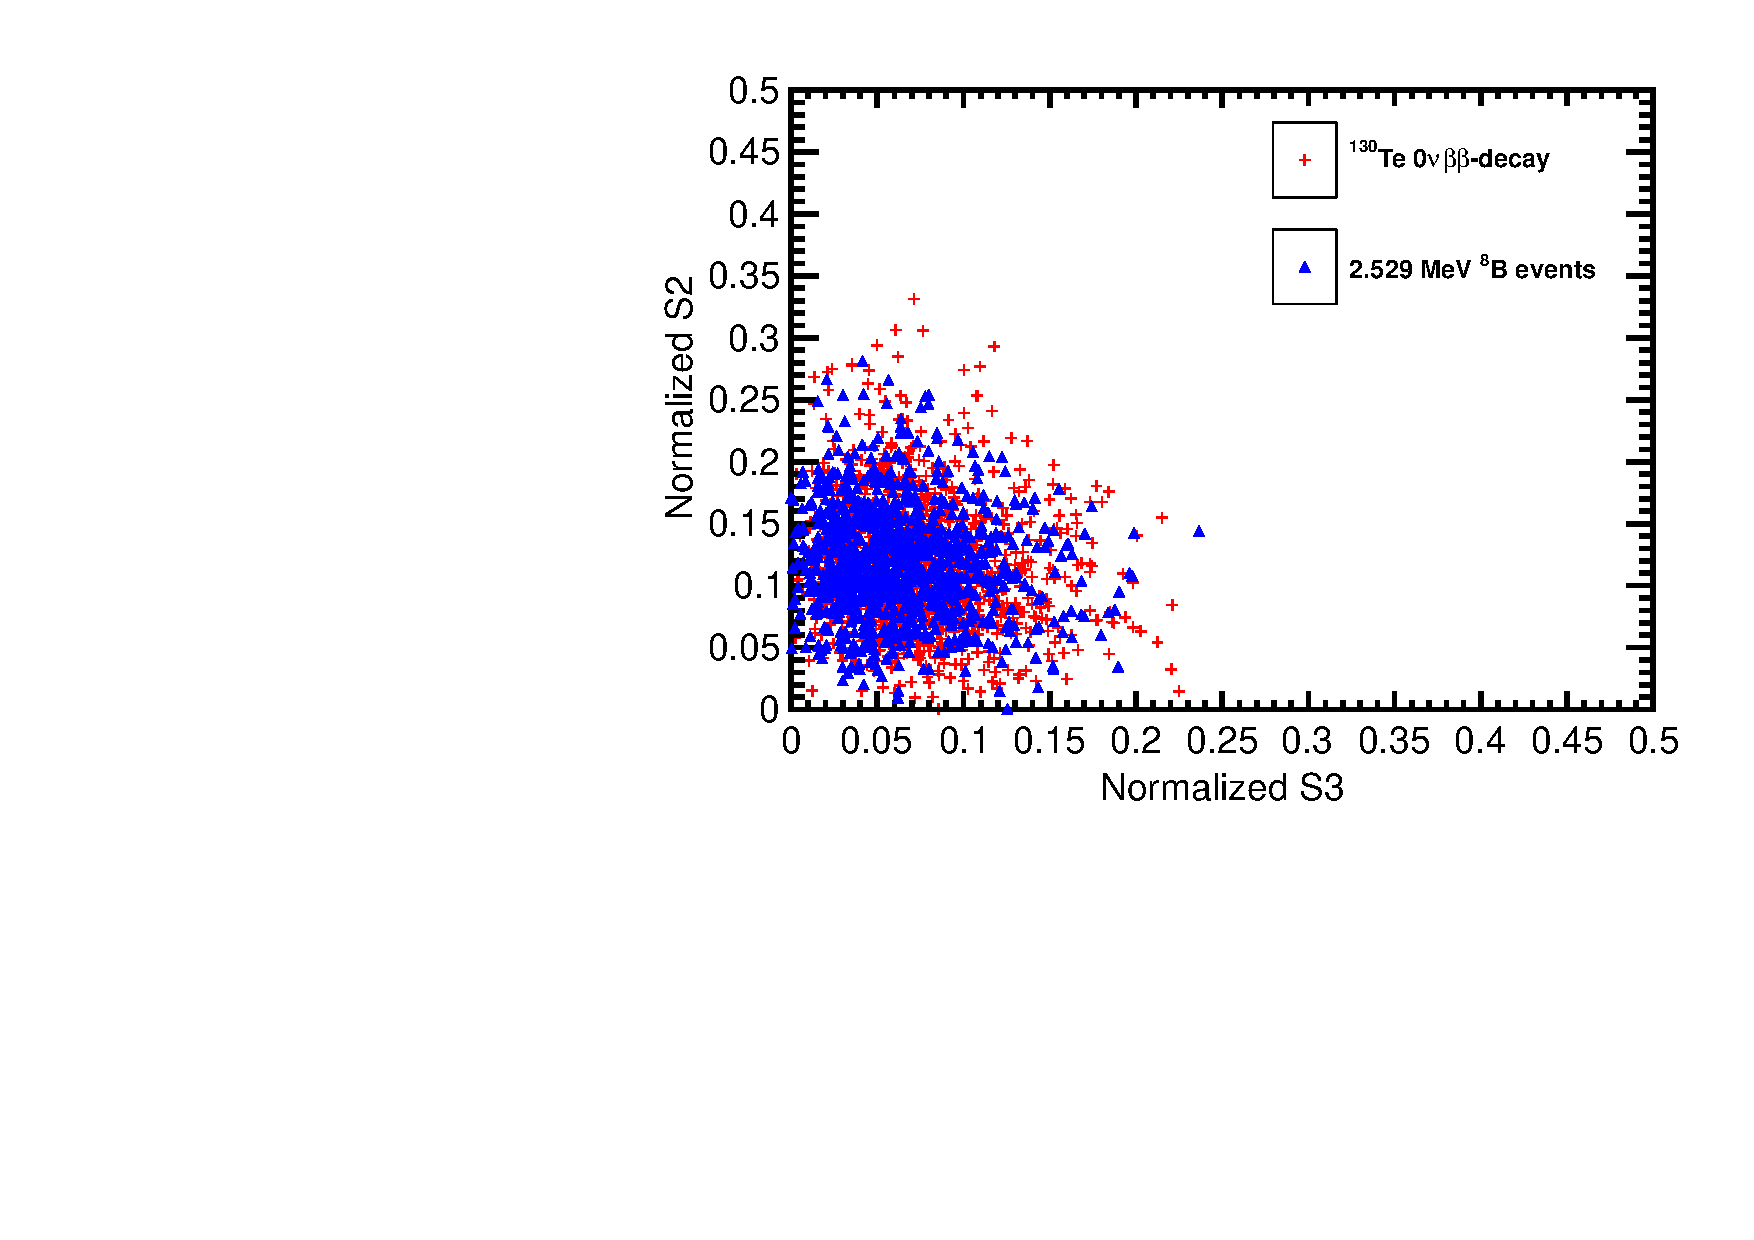
\includegraphics[width=0.49\textwidth]{hS2vsS3_Te130_1el_allLight_VtxSmear0cm_VtxShiftX0cm_33p5ns_center.pdf}
  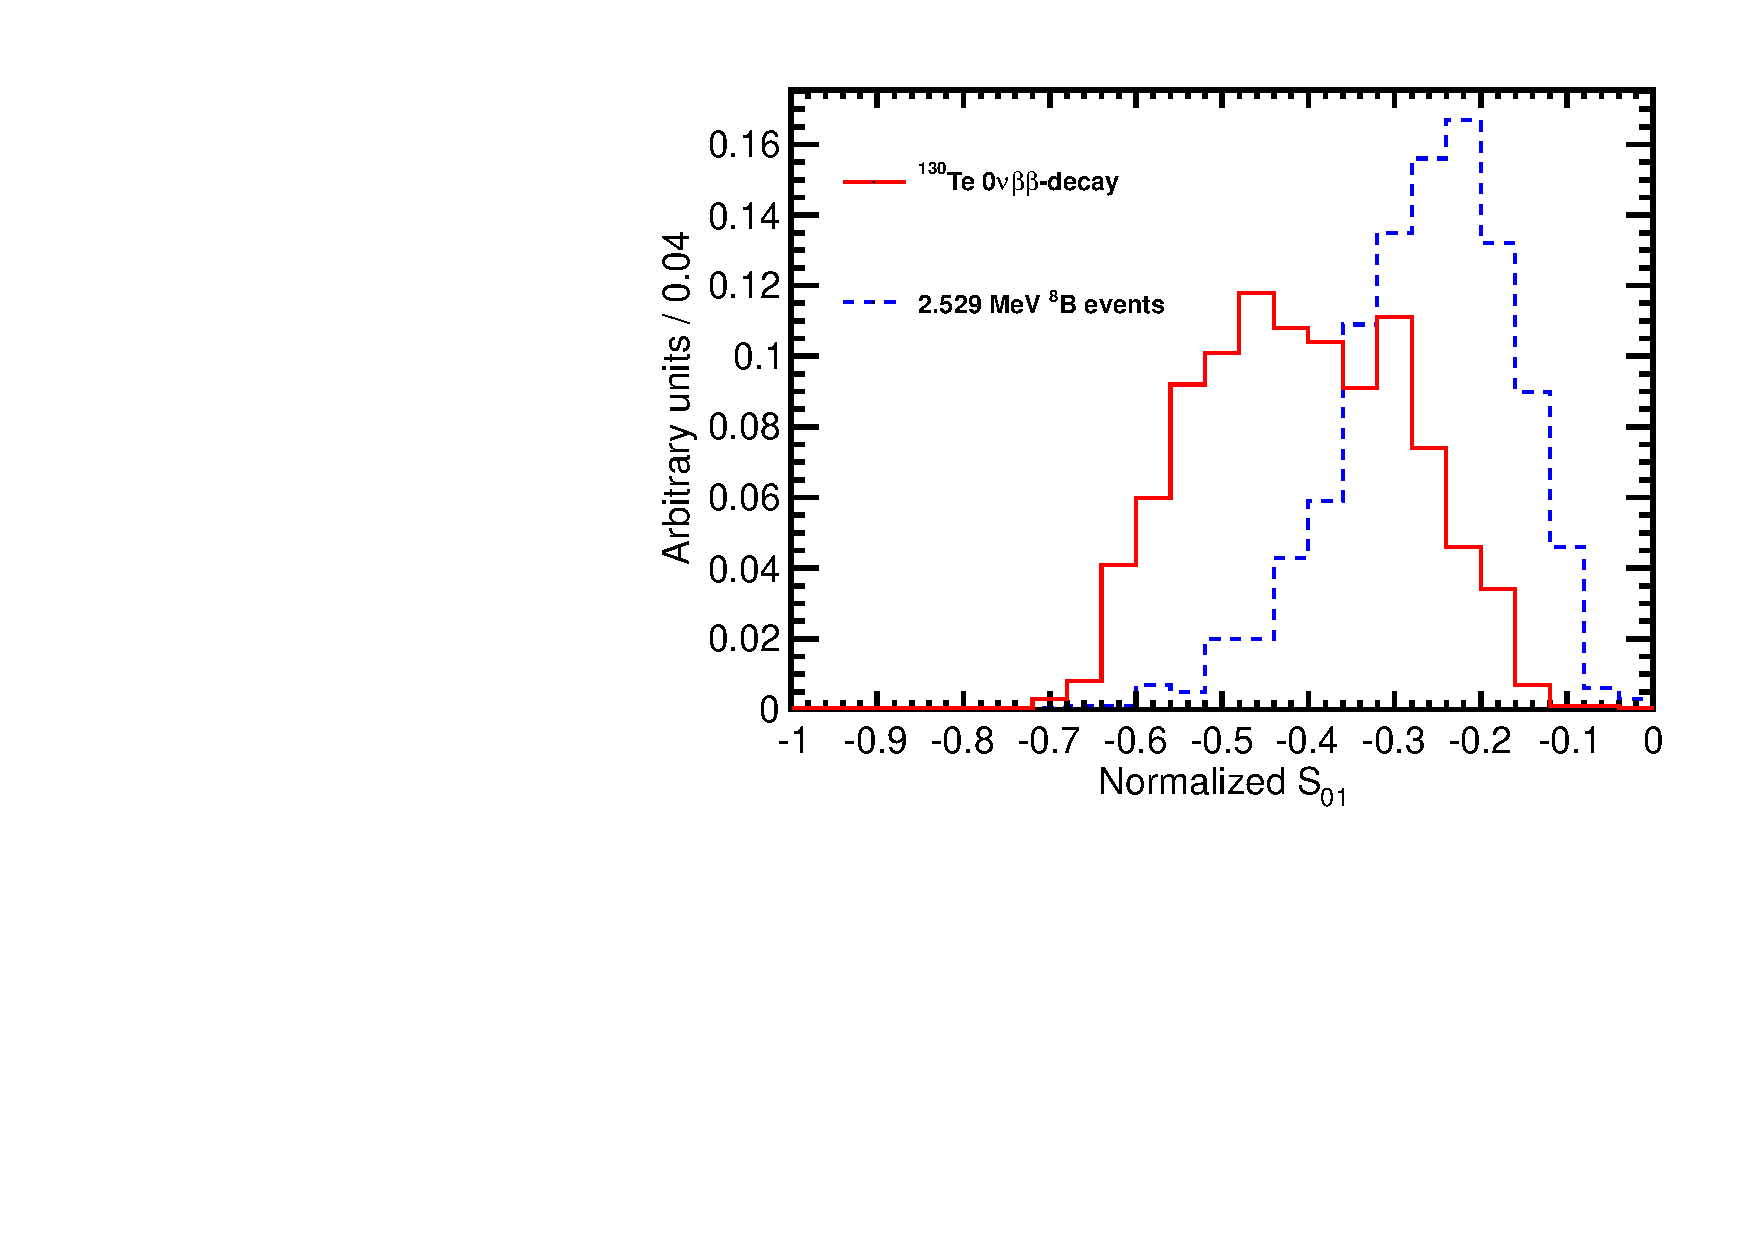
\includegraphics[width=0.9\textwidth]{hS01_allLight_VtxSmear0cm_VtxShiftX0cm_33p5ns_center.pdf}
  \caption{Spherical harmonics comparison between $^{130}$Te 0{\nbb}
    decay signal ($Q=2.529$~MeV) (\emph{red}) and $^{8}$B solar
    neutrinos background (\emph{blue}) for 1000 simulated events
    originated at the center of the sphere. $^{8}$B events are
    implemented as 2.529~MeV electrons with initial direction along
    $x$-axis. Perfect vertex reconstruction - true vertex position is
    used. Time cut of 33.5~ns on the photon arrival time is
    applied. \emph{Top left:} $S_0$ versus $S_1$ scatter plot. Black
    dotted line is a linear fit of these 2D histograms. Variable
    $S_{01}$ is defined as a projection of 2D distribution onto this
    linear fit. \emph{Top right:} $S_2$ versus $S_3$ scatter
    plot. \emph{Bottom:} $S_{01}$ distribution for the signal and
    background.}
\label{fig:SL_Te_33p5ns_center}
\end{figure*}


\subsection{Experimental challenges}

So far only events at the center of the detector have been
considered. In this section we discuss performance of the spherical
harmonics analysis for events distributed within the fiducial volume
of the detector taking into account finite resolution on vertex
position reconstruction.

When the vertex is not at the center, a uniform time cut on the photon
arrival time is no longer effective in the selection of Cherenkov
photons. In the case of off-center vertex, even significantly delayed
scintillation photons can reach the side of the detector that is
closer to the vertex much earlier than Cherenkov photons traveling to
the opposite side of the detector. Therefore, the time cut has to be
position dependent and take into account the total distance traveled
by each individual photon.

We found that the time cut defined as $\Delta t=t^{phot}_{measured} -
t^{phot}_{predicted}<$1~ns selects photons with sufficient fraction of
Cherenkov photons. Predicted time, $ t^{phot}_{predicted}=l/v^{phot}$,
depends on total distance, $l$, traveled by the photon and proper
assignment of the velocity for each photon, $v^{phot}$, that depends
on index of refraction, (Note, we use average index of refraction of
n=1.53). Therefore the relative Cherenkov/scintillation composition of
the light selected with this $\Delta t$ time cut depends on the vertex
location and chromatic dispersions.

Due to chromatic dispersion, even with perfect vertex reconstruction
one cannot achieve the same level of separation between Chrerenkov and
scintillation light compared to the central events considered above in
Section 4. This in turn reduces the effectiveness of the spherical
harmonics analysis in separating of 0{\nbb} decay and $^{8}$B events
(see Fig.~\ref{fig:SL_Te_SmearX0cm_momDT1ns_rndVtx_3p0m}). However
next generation detectors can recover losses due to chromatic
dispersion by choosing liquid scintillators with a more narrow
emission spectrum.


\begin{figure*}[h]
  \centering
  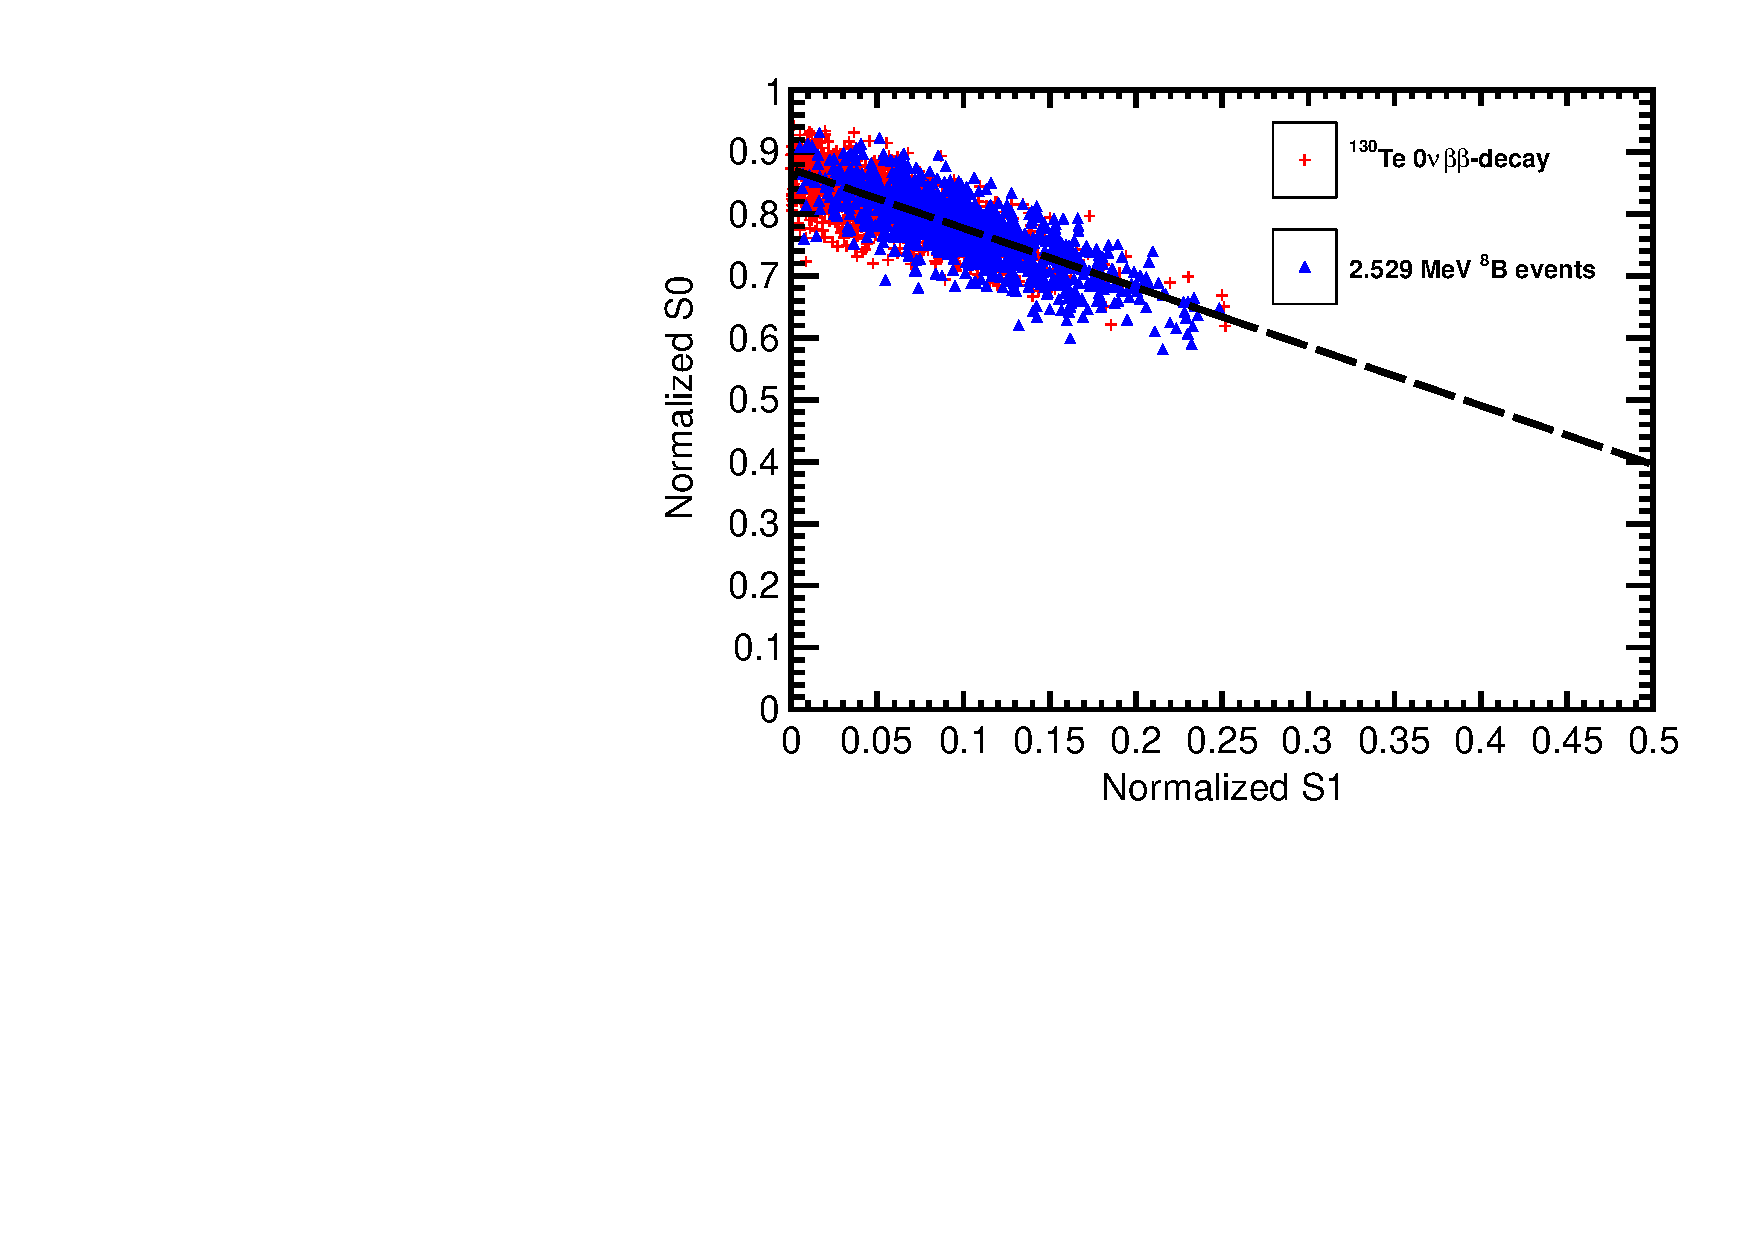
\includegraphics[width=0.49\textwidth]{hS0vsS1_Te130_1el_allLight_VtxSmear0cm_VtxShiftX0cm_momDT1p0ns_rndVtx_3p0mSphere.pdf}
  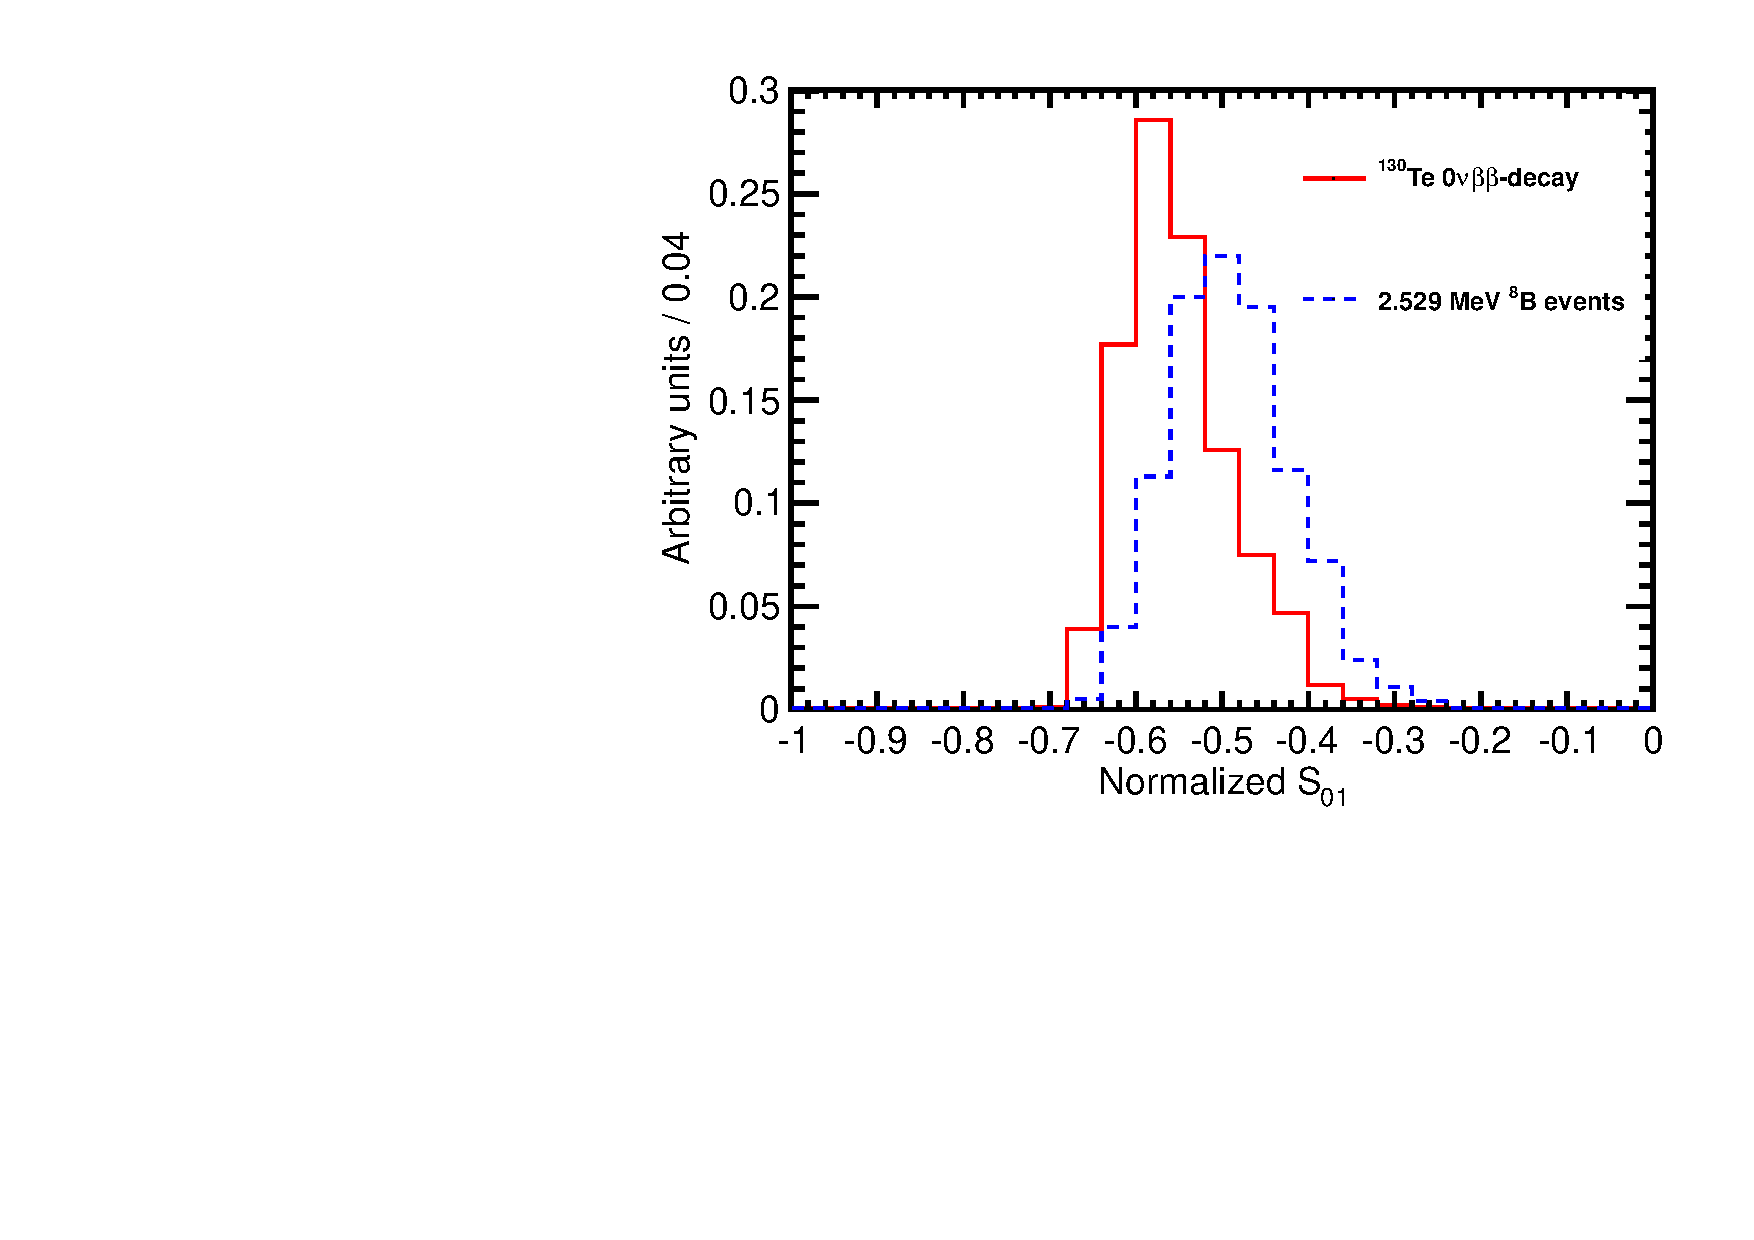
\includegraphics[width=0.49\textwidth]{hS01_allLight_VtxSmear0cm_VtxShiftX0cm_momDT1p0ns_rndVtx_3p0mSphere.pdf}
  \caption{Spherical harmonics comparison between $^{130}$Te 0{\nbb}
    decay signal ($Q=2.529$~MeV) (\emph{red}) and $^{8}$B solar
    neutrinos background (\emph{blue}) for 1000 simulated
    events.Verticies are uniformly distributed within the fiducial
    volume, $R<3$~m. $^8$Be events are implemented as 2.529~MeV
    electrons with the initial momentum direction uniformly
    distributed within 4$\pi$ solid angle. Perfect vertex
    reconstruction - true vertex position is used. \emph{Left:} $S_0$
    versus $S_1$ scatter plot. Black dotted line is a linear fit of
    these 2D histograms. Variable $S_{01}$ is defined as a projection
    of 2D distribution onto this linear fit. \emph{Right:} $S_{01}$}
  \label{fig:SL_Te_SmearX0cm_momDT1ns_rndVtx_3p0m}
\end{figure*}



Imprecise knowledge of the vertex position due to finite resolution is
another factor affecting performance of the spherical harmonics
analysis. Small deviations in vertex reconstruction cause large effect
on $S_0$ and $S_1$ for single electron event topology. For the
verticies shifted along the direction of the electron the $\Delta t$
cut makes uniform scintillation light distribution less uniform. The
$\Delta t$ cut selects more forward emitted photons in the case when
the reconstructed vertex is shifted to the direction opposite to the
electron momentum (enhancing forward region populated by Cherenkov
photons - more asymmetric photon distribution causing higher values of
$S_1$). It selects more backward emitted photons in the case when the
reconstructed vertex is shifted in the direction along the electron
momentum (counter balancing forward region populated by Cherenkov
photons - more symmetric photon distribution causing smaller values of
$S_1$).

\begin{figure*}[h]
  \centering
  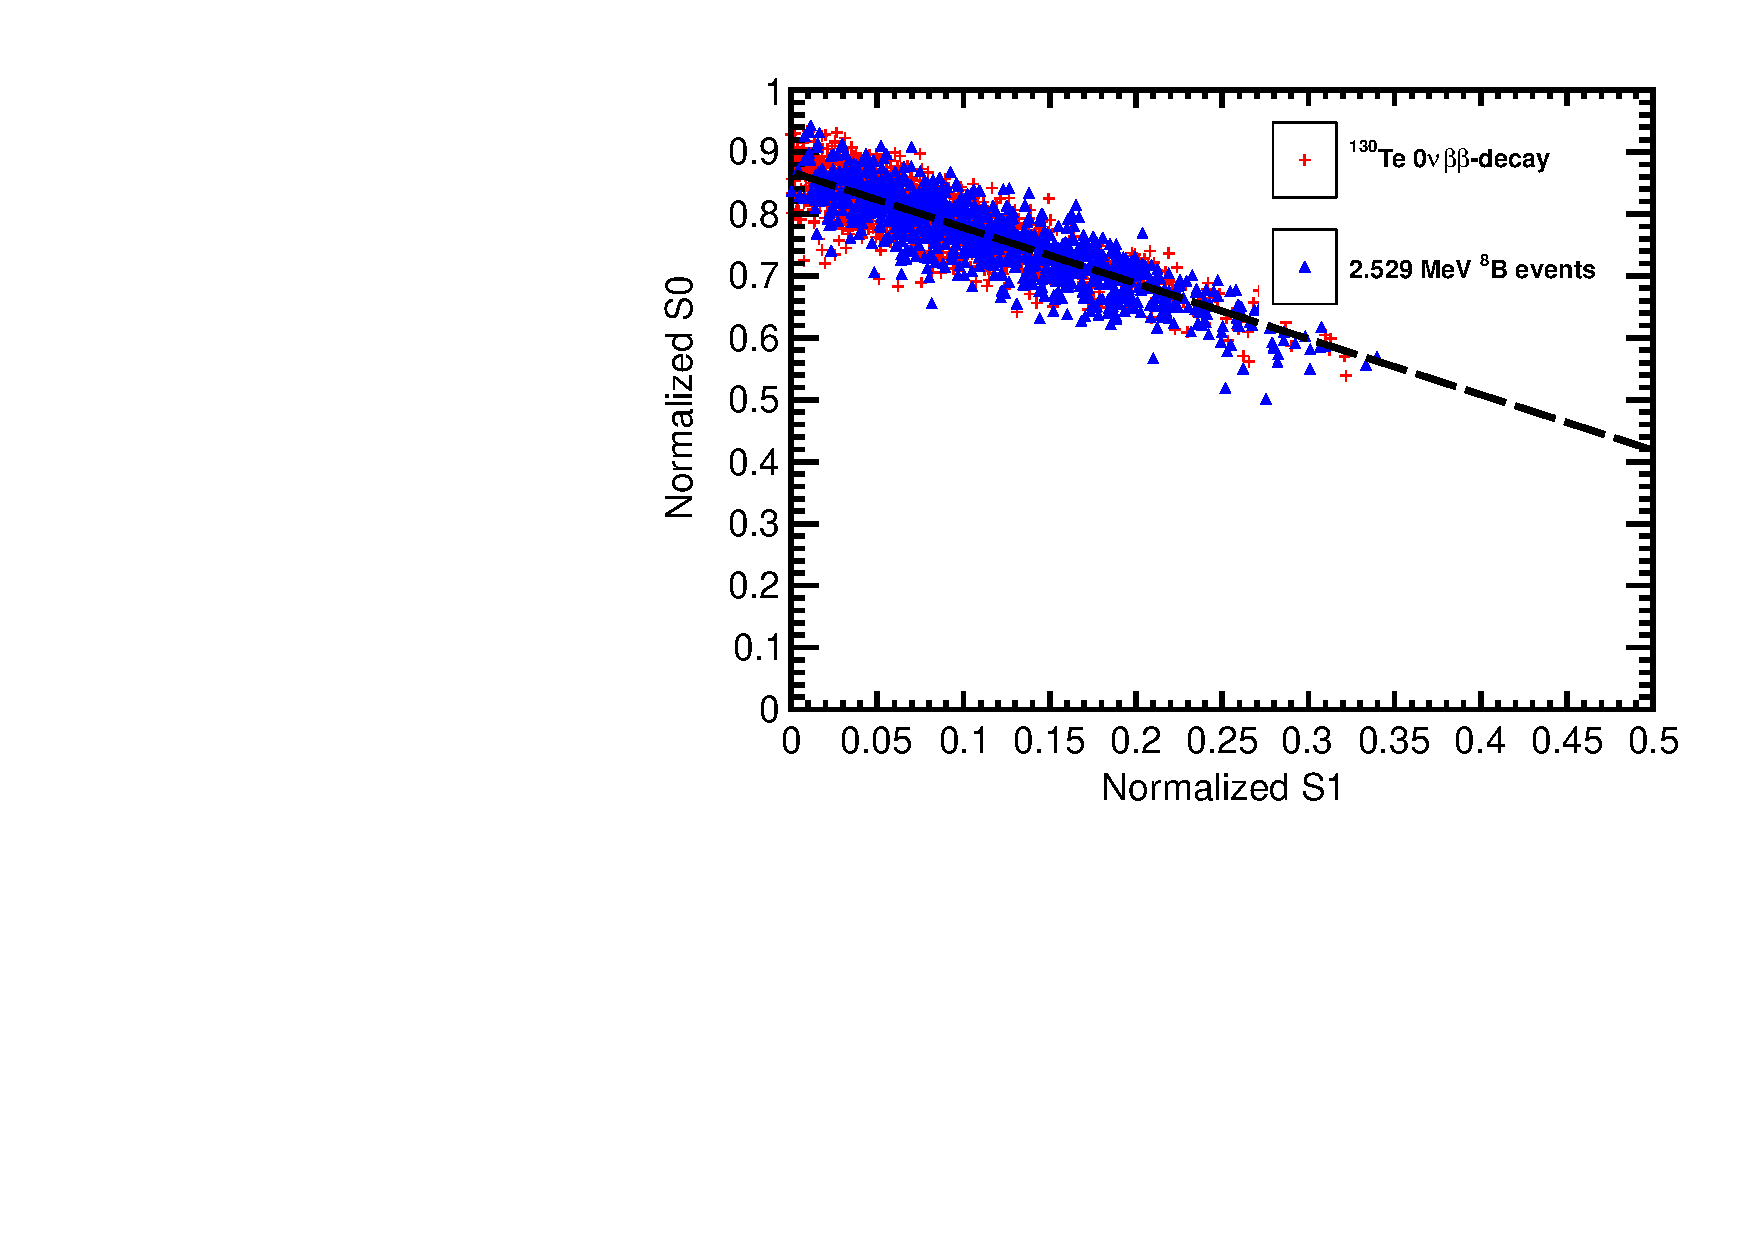
\includegraphics[width=0.49\textwidth]{hS0vsS1_Te130_1el_allLight_VtxSmear3cm_VtxShiftX0cm_momDT1p0ns_rndVtx_3p0mSphere.pdf}
  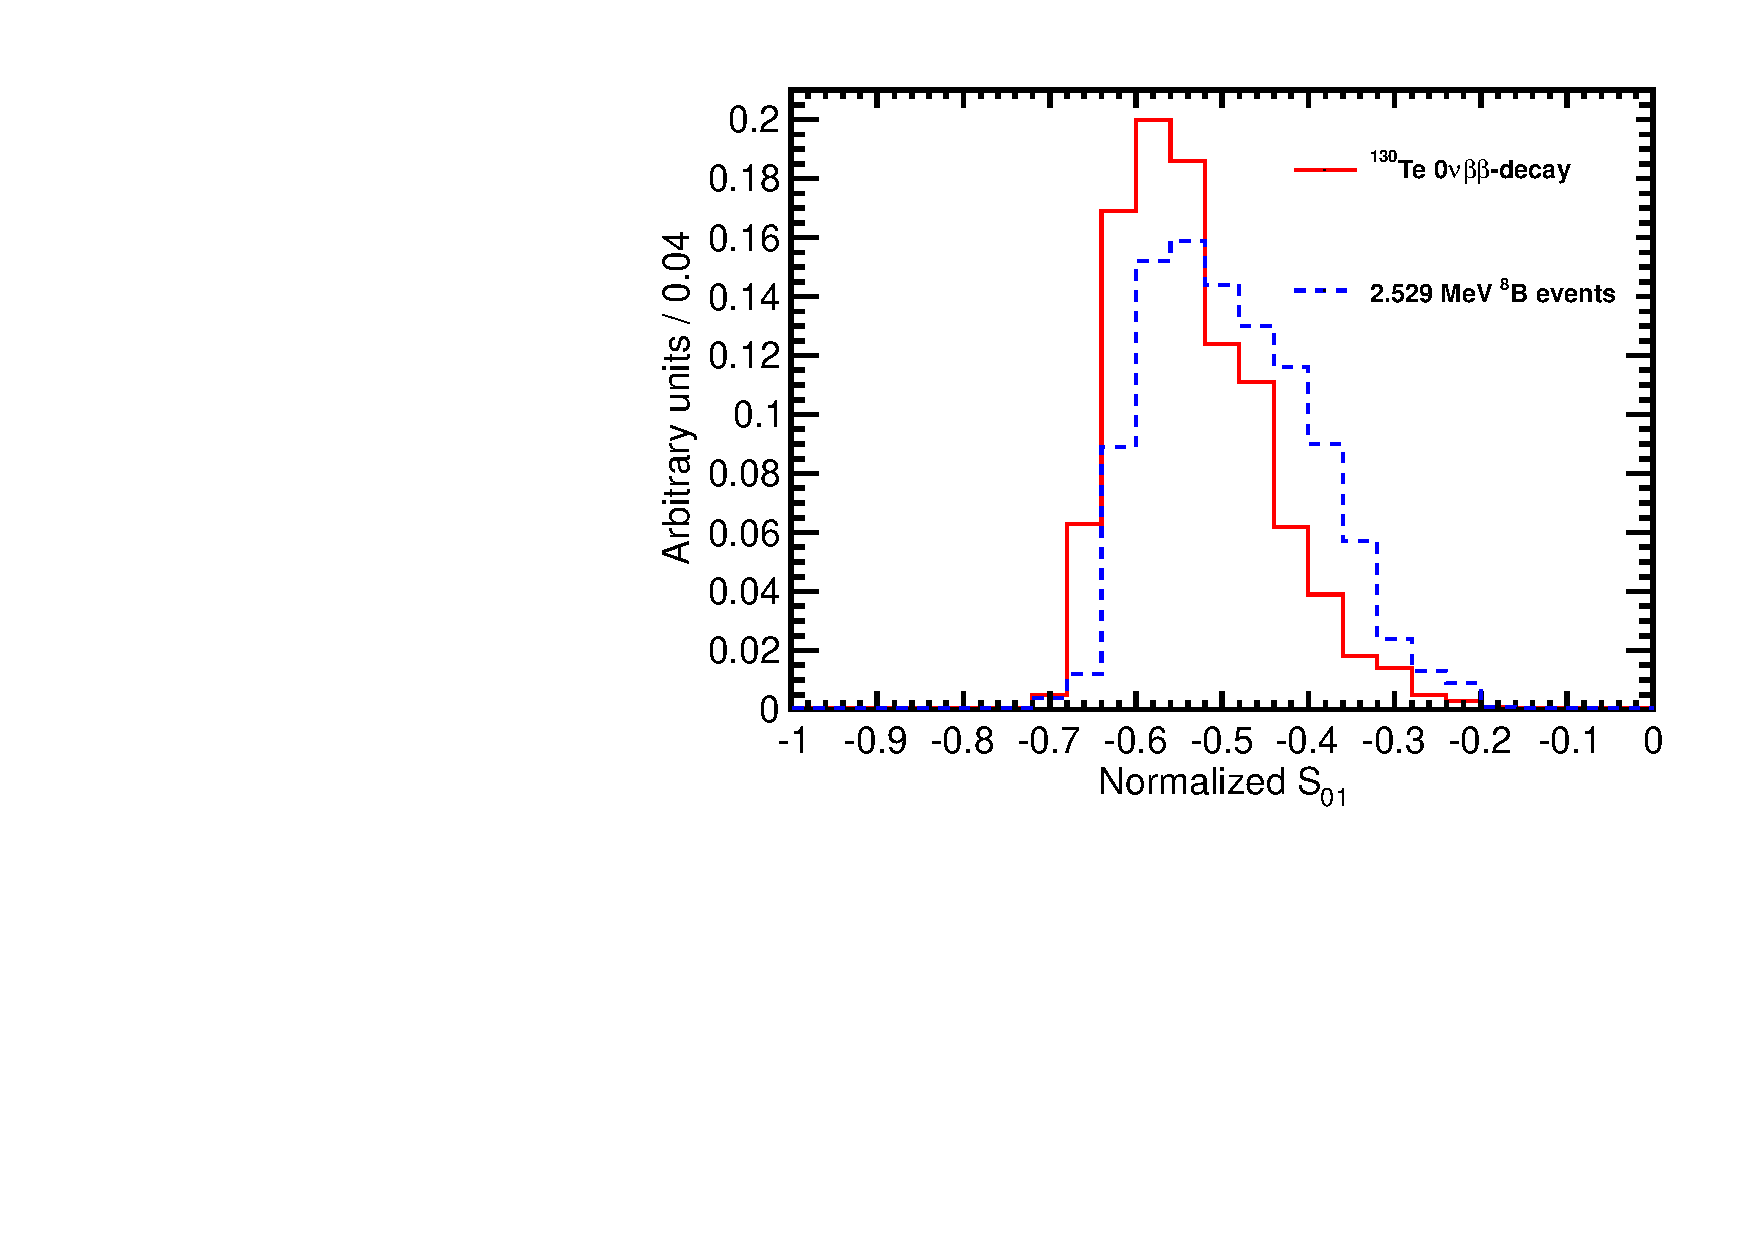
\includegraphics[width=0.49\textwidth]{hS01_allLight_VtxSmear3cm_VtxShiftX0cm_momDT1p0ns_rndVtx_3p0mSphere.pdf}
  \caption{Spherical harmonics comparison between $^{130}$Te 0{\nbb}
    decay signal ($Q=2.529$~MeV) (\emph{red}) and $^{8}$B solar
    neutrinos background (\emph{blue}) for 1000 simulated
    events.Verticies are uniformly distributed within the fiducial
    volume, R$<$3~m. $^8$Be events are implemented as 2.529~MeV
    electrons with the initial momentum direction uniformly
    distributed within 4$\pi$ solid angle. Vetrex is smeared with 3~cm
    resolution. \emph{Left:} $S_0$ versus $S_1$ scatter plot. Black
    dotted line is a linear fit of these 2D histograms. Variable
    $S_{01}$ is defined as a projection of 2D distribution onto this
    linear fit. \emph{Right:} $S_{01}$}
\label{fig:SL_Te_SmearX3cm_momDT1ns_rndVtx_3p0m}
\end{figure*}


{\bf Solution to this problem would be a better selection criteria of
  early light. It has to preserve high admixture of the Cherenkov
  photons, but needs to select scintillation photons in a more uniform
  manner. Working on it, but may not be simple so I don't want to
  include it in this paper.}

Good vertex resolution is essential for spherical harmonics
analysis. Such strong dependence on the vertex resolution can be
addressed by choosing a different liquid scintillator mixture with a
more delayed emission of the scintillation
light. Figure~\ref{fig:SL_Te_momDT1ns_sci0p5ns_rndVtx_3p0m} shows
spherical harmonics calculated for the time profile which has
scintillation component delayed by 0.5ns with respect to what is shown
in Fig.~\ref{fig:Arrival_time}


\begin{figure*}[h]
  \centering
  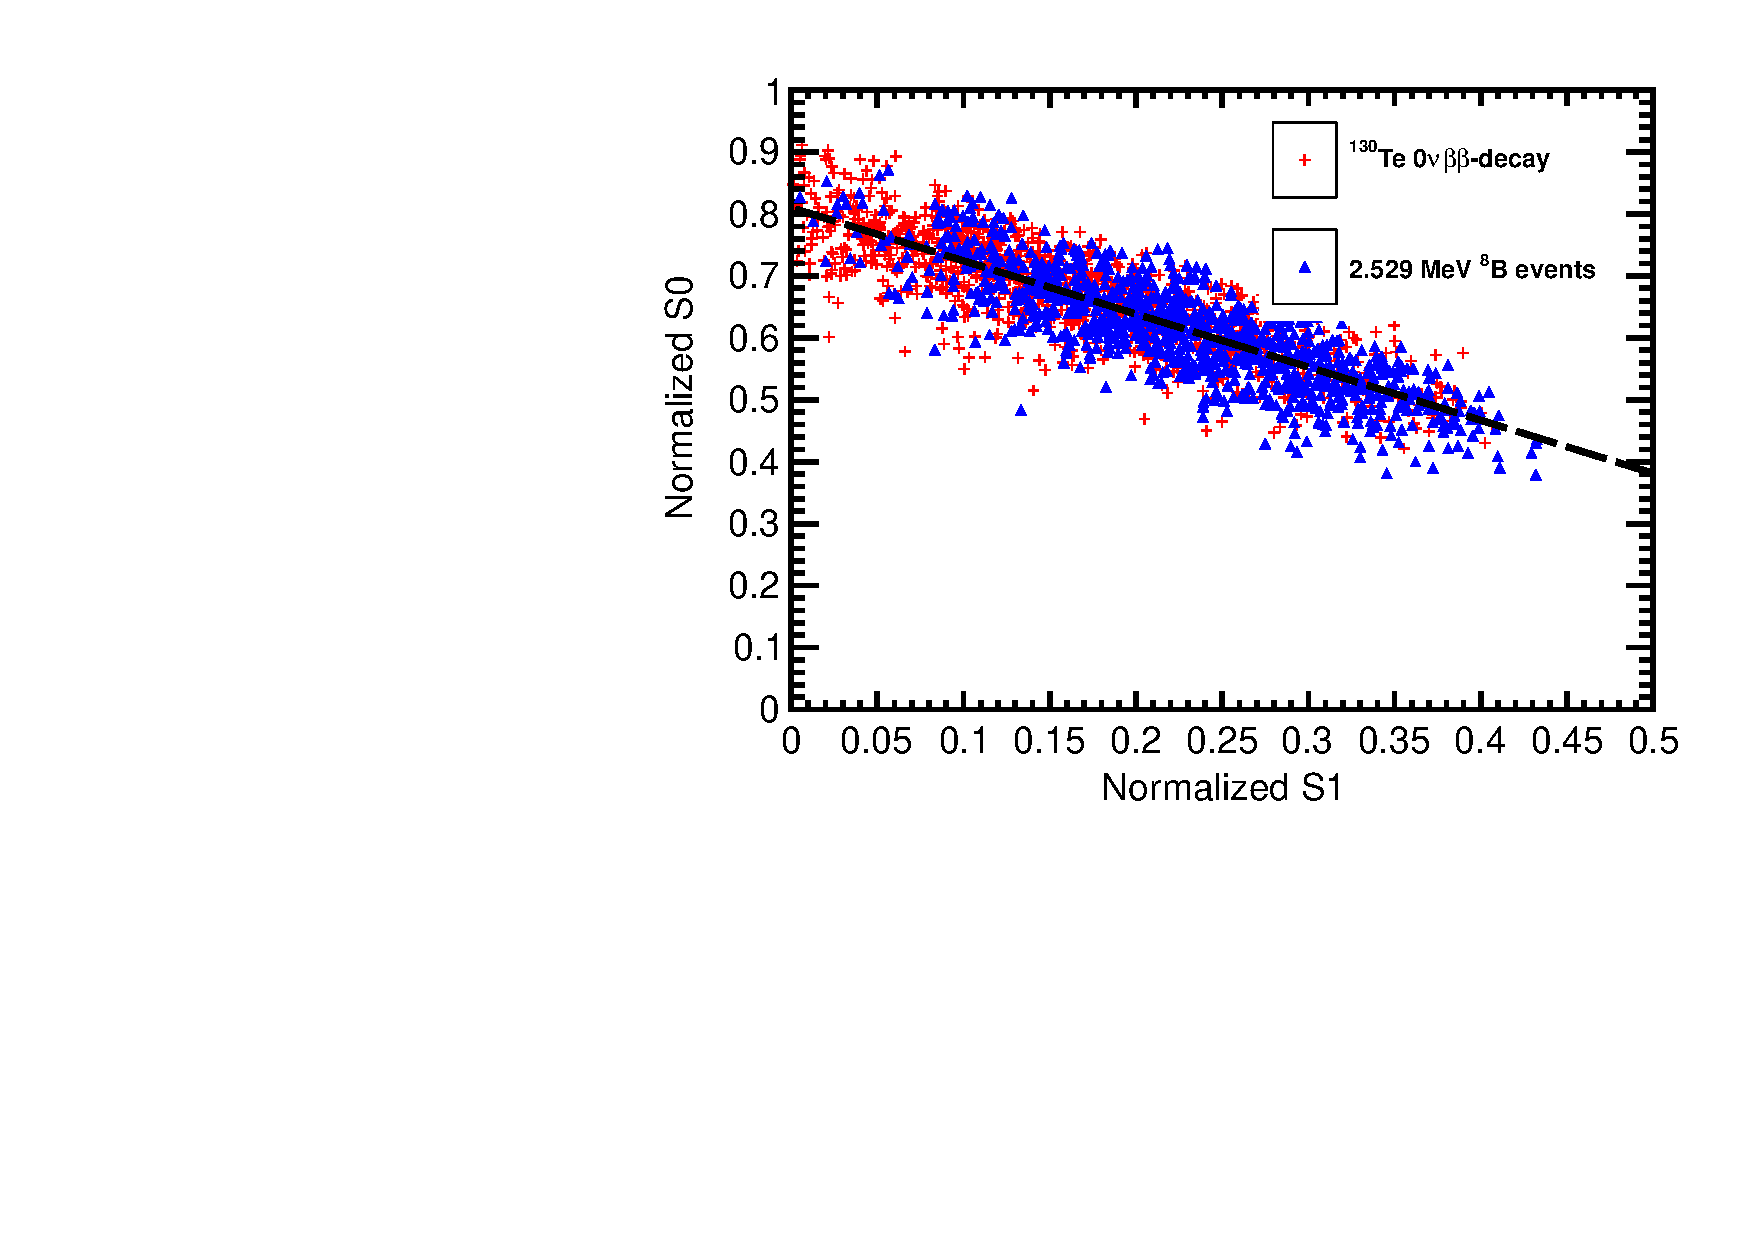
\includegraphics[width=0.49\textwidth]{hS0vsS1_Te130_1el_allLight_VtxSmear3cm_VtxShiftX0cm_momDT1p0ns_sci0p5ns_rndVtx_3p0mSphere.pdf}
  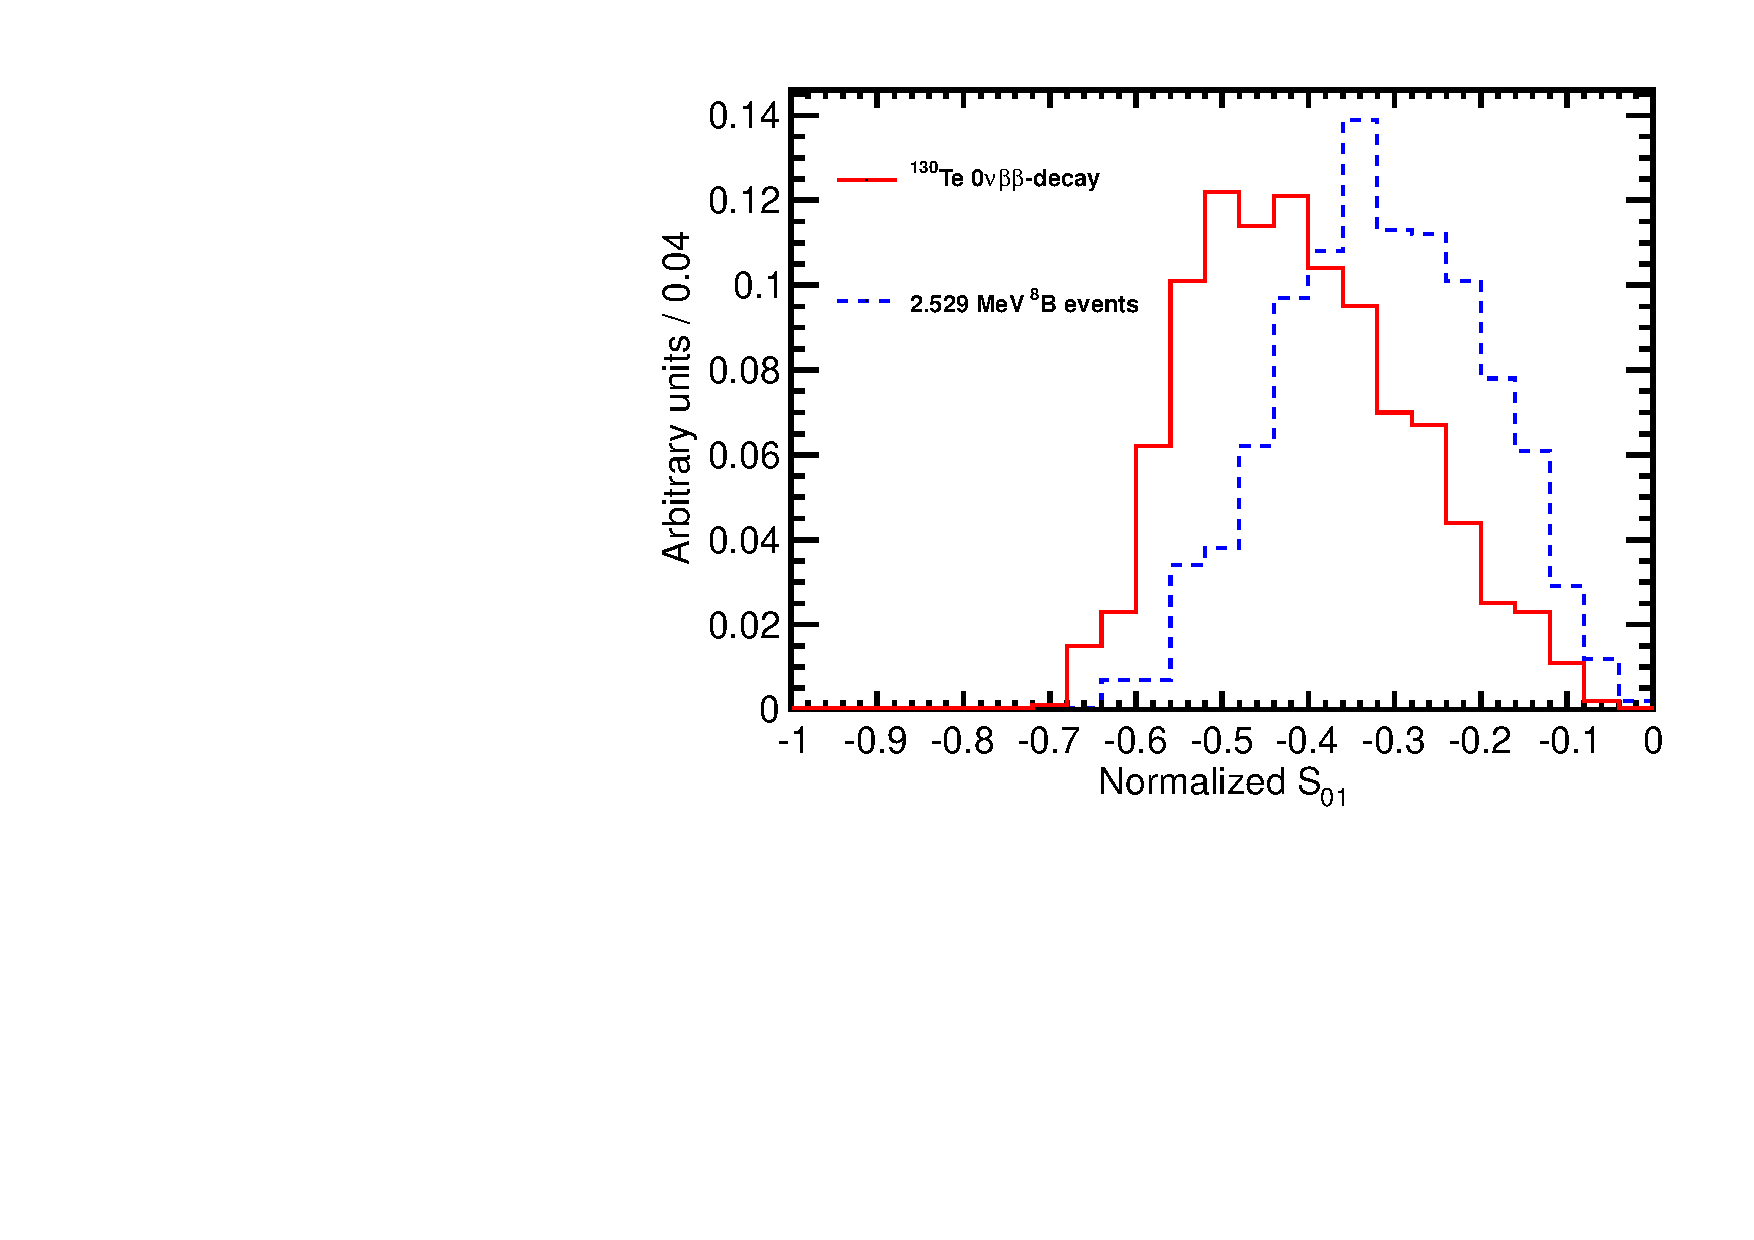
\includegraphics[width=0.49\textwidth]{hS01_allLight_VtxSmear3cm_VtxShiftX0cm_momDT1p0ns_sci0p5ns_rndVtx_3p0mSphere.pdf}
  \caption{Spherical harmonics comparison between $^{130}$Te 0{\nbb}
    decay signal ($Q=2.529$~MeV) (\emph{red}) and $^{8}$B solar
    neutrinos background (\emph{blue}) for 1000 simulated
    events. Verticies are uniformly distributed within the fiducial
    volume, $R<3$~m. $^8$Be events are implemented as 2.529~MeV
    electrons with the initial momentum direction uniformly
    distributed within 4$\pi$ solid angle. Vetrex is smeared with 3~cm
    resolution. {\bf Scintillation light is delayed by additional
      0.5~ns.} \emph{Left:} $S_0$ versus $S_1$ scatter plot. Black dotted
    line is a linear fit of these 2D histograms. Variable $S_{01}$ is
    defined as a projection of 2D distribution onto this linear
    fit. \emph{Right:} $S_{01}$}
\label{fig:SL_Te_SmearX3cm_momDT1ns_sci0p5ns_rndVtx_3p0m}
\end{figure*}

